\documentclass[a4paper,12pt]{article} 
\usepackage[utf8x]{inputenc} 
\usepackage[french]{babel} 
\usepackage[colorlinks=true,urlcolor=blue,linkcolor=blue]{hyperref}
\usepackage{fullpage}
\usepackage{url}
\usepackage{a4wide}
\usepackage{graphicx}
\usepackage{float}
\usepackage[toc,page]{appendix}

\renewcommand{\appendixtocname}{Annexes}
\renewcommand{\appendixpagename}{Annexes} 
\addto\captionsfrench{\def\tablename{{Tableau}}}
\begin{document}

\title{Analyse des besoins et tests pour le projet\\
  \textit{Réalisation d'un jeu d'Othello}}

\author{Morgane Badré\\
  Benjamin Letourneau,\\
  Vincent Wilmet,\\
  Nicolas Yvon\\}
\date{}

\maketitle

Ce document présente l'analyse des besoins pour le projet de Réalisation d'un jeu d'Othello. Deux types de besoins seront étudiés:

\section{Besoins fonctionnels}

Les besoins fonctionnels sont des besoins en rapport direct avec les
demandes de l'utilisateur. Des diagrammes UML accompagnent ces
spécifications afin de simplifier l'analyse (annexes \ref{A}, \ref{B},
\ref{C}). Les fonctionnalités sont classées par priorité de développement.

\subsection{Jouer une partie / mettre en pause une partie}
L’utilisateur doit pouvoir lancer à tout moment une partie avec l'affichage d'un plateau contenant l’environnement initial, ainsi que faire une pause dans le déroulement de la partie. Le lancement d'une partie ne doit pas prendre plus de 2 secondes. Cette fonctionnalité ne sera pas difficile à implémenter.

\begin{description}
\item[Test système] Appuyer sur le bouton lance bien le mode Jeu du logiciel.
\end{description}

\subsection{Réaliser une Intelligence Artificielle (IA) }
\label{IA}
L'utilisateur doit pouvoir jouer contre une Intelligence Artificielle tout d'abord naïve puis plus tard, si possible, évolutive. L'IA doit pouvoir apporter une solution en un temps imparti par l'utilisateur. Le risque de cette approche est que l'IA peut être très longue à répondre selon l'avancée de la partie. Dans ce cas, l'algorithme le plus adapté sera choisi et un compteur de temps sera ajouté pour empêcher tout débordement sur le temps maximal. Cette fonctionnalité est certainement la plus difficile du projet.

\begin{description}
\item[Test comportemental] Vérifier que le résultat de la réflexion de l’IA est correct.
\item[Test de performance] Exécuter le logiciel en même temps qu’un autre (gourmand en ressources) afin de voir si les résultats obtenus sont identiques sur une même partie. (savoir si l’IA est compétente).
\end{description}

\subsection{Enregistrer une partie / Relancer une partie}
L'utilisateur doit pouvoir enregistrer sa partie et la relancer pour pouvoir la continuer. Cette action est réalisée à travers l’actionnement d’un bouton. Le fichier de sauvegarde doit être créé en moins de 5 secondes et ne doit pas dépasser une taille de 10 Ko. Il sera nécessaire d'implémenter un petit analyseur syntaxique et lexical pour la lecture et l'écriture des fichiers de sauvegarde. Les risques de cette fonctionnalité sont qu'il est possible que la sauvegarde soit interrompue et donc qu'il y ait une perte de données, le fichier étant alors corrompu. Ce risque peut être paré par une protection des données du fichier par l'utilisation de balises ouvrantes et fermantes afin de vérifier l'intégrité des données du fichier. Cette fonctionnalité sera facile à implémenter.

\begin{description}
\item[Test système] Le fichier de sauvegarde est bien créé et valide. Le plateau affiché correspond bien au fichier en entrée.
\item[Test aléatoire] Lancer aléatoirement des enregistrements de la partie.
\end{description}

\subsection{Recommencer une partie à une certaine position}
L’utilisateur doit pouvoir recommencer à jouer à une partie, préalablement lancée et enregistrée, en ayant la possibilité de choisir à partir de quel état du plateau recommencer. C’est-à-dire que si 10 coups ont été joués alors l’utilisateur peut choisir de recommencer à partir du deuxième ou bien du huitième. Ainsi, le fichier de sauvegarde doit contenir un historique complet de la partie en l'état. Le temps de chargement d'un fichier de sauvegarde et la mise en place du plateau à la position souhaitée ne doit pas prendre plus de 10 secondes. En cas de crash de la sauvegarde, le système récupèrera l'avant-dernière sauvegarde. Celle-ci a une difficulté d'implémentation normale.

\begin{description}
\item[Test unitaire] La position choisie correspond bien à celle sauvegardée.
\item[Test négatif] Choisir une position hors des bornes de la partie ($<$ 0 ou $>$ au dernier coup).
\end{description}

\subsection{Possibilité de revenir un coup en arrière}

L’utilisateur doit pouvoir, s’il a effectué un déplacement non désiré, revenir en arrière dans le jeu afin de rejouer les coups qu’il désire (mécanisme Défaire/Refaire). L'utilisateur aura le choix parmi tous les coups qu'il avait joués et pourra ainsi revenir en arrière pour tester une stratégie différente. Le temps de modification de l'affichage et de la structure doit être quasi-instantané, une demi-seconde. Une corruption éventuelle d'historique conduit à utiliser l'historique du coup précédent. Il faudra donc garder en mémoire tous les coups joués et permettre de ``revenir en avant'', c'est-à-dire, annuler un retour en arrière. Cette fonctionnalité a une difficulté d'implémentation normale.

\begin{description}
\item[Test unitaire] La position choisie correspond bien à celle sauvegardée.
\item[Test aux limites] Cette fonctionnalité doit être désactivée lorsque qu’il n’y a plus aucun coup précédant le coup actuel.
\item[Test aléatoire] Simulation d'un nombre aléatoire de retours en arrière.
\end{description}

\subsection{Fournir le manuel utilisateur du jeu (interface et règles)}

L'utilisateur doit pouvoir accéder à une aide générale sur le fonctionnement et les règles du jeu. Cette aide sera introduite par l’ouverture d’un fichier PDF qui pèsera moins de 10 Mo. L'explication sera lisible et assimilable en moins de 10-15 minutes. Il faudra alors résumer pour mettre l'essentiel et vulgariser les explications afin qu'elle soit compréhensible par tous. Cette fonctionnalité sera facile à réaliser.

\begin{description}
\item[Test unitaire] Le PDF de l’aide s’affiche bien lors de l’appui sur le bouton.
\end{description}

\subsection{Proposer des suggestions de coups par l'IA}

L’utilisateur doit pouvoir demander au logiciel de l’aide pour visualiser le meilleur coup à jouer après analyse par l’IA qui proposera plusieurs niveaux d'aide comme par exemple, le choix entre les deux meilleurs coups à jouer. L'IA doit répondre en un temps acceptable dans l'ordre de 2 à 3 secondes. L'algorithme utilisé dépendra de l'avancement de la partie. Pour que l'algorithme choisi ne prenne pas trop de temps, on ajoutera un compteur de temps. La difficulté de cette fonctionnalité dépendra de la difficulté de l'intégration de l'IA (voir fonctionnalité n°\ref{IA}).

\begin{description}
\item[Test unitaire] Cette fonctionnalité doit toujours nous renvoyer une position correspondant à un coup valide.
\item[Test aux limites] Ce bouton n'est activé que lorsque le joueur peut jouer.
\end{description}

\subsection{Chargement d’un fichier pré-configuré}

L’utilisateur doit pouvoir sélectionner un fichier qu’il a composé afin de jouer sur un plateau de sa configuration. Ce fichier doit être écrit de façon interprétable par le logiciel. Le fichier doit être vérifié et chargé puis le plateau qui en résulte doit être affiché en 5 secondes maximum. Le fichier peut-être corrumpu donc une vérification de jalons de début et de fin obligatoire ainsi que la présence des informations requises permettra de parer à ce risque. S'il y a corruption du fichier ou une erreur lors de la position des jetons dans le fichier, un message d'erreur s'affichera. Cette fonctionnalité n'est pas dure à implémenter.

\begin{description}
\item[Test système] Le plateau correspond bien au fichier entré si celui-ci est valide.
\end{description}

\subsection{Possibilité de choisir la taille de la grille de jeu}

L'utilisateur doit pouvoir choisir la taille de sa grille de jeu. C'est-à-dire une grille 5*5, 6*6, ... Ou plus. Mais aussi 6*10, ou autre grille rectangulaire. La grille pourra être choisie dans une limite d'au minimum 3x3 jusqu'au maximum 50x50. Le risque de cette fonctionnalité est que l'utilisateur choisisse une grille trop grande ou trop petite pour que le logiciel soit jouable. Il suffira de limiter la taille de la grille et d'obliger l'utilisateur à entrer les bonnes dimensions. Cette fonctionnalité est simple à implémenter.

\begin{description}
\item[Test unitaire] La grille doit correspondre à la taille demandée.
\item[Test négatif] La grille ne doit pas être acceptée si la taille demandée est trop grande ou trop petite.
\item[Test aléatoire] Lancer différentes configurations de grilles qui soient dans l’intervalle autorisé.
\end{description}

\subsection{Menu pour choisir le temps de réflexion de l’IA}

Le joueur doit pouvoir choisir si l’IA prendra plus ou moins beaucoup de temps pour le calcul des coups. Ce temps ne devra pas pouvoir dépasser 2 jours. Cette fonctionnalité ne devrait pas poser de problème particulier.

\begin{description}
\item[Test système] Le temps de réflexion de l’IA doit correspondre à celui donner dans le menu de la partie.
\item[Test aléatoire]  Entrer des temps aléatoires raisonnables, < 3 secondes, pour le temps de réflexion de l’IA et vérifier que l’algorithme le respecte.
\end{description}


\subsection{Possibilité d’échanger les joueurs}

Le logiciel doit permettre au joueur d’échanger sa place avec l’IA et de pouvoir continuer la partie ainsi. Le temps de réponse du logiciel pour échanger les joueurs ne doit pas dépasser plus de 2 secondes. Il ne sera possible d'échanger les joueurs que lorsque la partie aura été commencée et non terminée. Cette fonctionnalité n'est pas dure à implémenter.

\begin{description}
\item[Test unitaire] Il est visuellement possible de voir que nos jetons sont échangés avec ceux de notre adversaire.
\item[Test aléatoire] Tester pendant une partie l’échange des joueurs à des intervalles aléatoires.
\end{description}

\section{Besoins non fonctionnels}

Les besoins non fonctionnels sont des besoins en rapport direct avec le comportement du logiciel et la gestion du projet.

\subsection{Besoins comportementaux}

\subsubsection{Performances}

Le logiciel doit pouvoir s'exécuter en 2-3 secondes maximum. L'algorithme force-brute (recherche exhaustive) doit pouvoir calculer une stratégie maximale de 4x4 en 15 minutes maximum (moyenne). Le temps de calcul de l'algorithme force-brute pour une grille 6x6 ou 8x8 étant considérablement plus élevé, l'utilisation d'algorithmes plus évolués devra être étudiée et expérimentée. Le logiciel ne doit pas dépasser une utilisation de la mémoire supérieure à 2Go.

\begin{description}
\item[Test système] Exécuter le logiciel sur différents types de machines de puissances différentes : petites machines (netBook, notebook), machines de bureau (PC de salon, PC portable moyen, c’est-à-dire avec un dual core + 4go de ram maxi), machines de jeu (Core i7, 16GO de ram, …).
\end{description}

\subsubsection{Fiabilité}

Le logiciel doit implémenter des sauvegardes régulières pour permettre à l’utilisateur de pouvoir reprendre une partie coupée. Ces sauvegardes doivent être intègres.
Le logiciel doit enregistrer au fur et à mesure les coups joués en tant que position (i,j) dans un fichier annexe afin de garder une trace des parties réalisées.
Afin de permettre à l’utilisateur de récupérer une partie en cours avant un crash quelconque de l’ordinateur ou une fermeture de l’application, la partie doit être régulièrement enregistrée afin de pouvoir être relancée.

\begin{description}
\item[Test système] Fermer l’application en plein milieu d’une partie, pendant le chargement d’une partie, pendant la réflexion de l’IA. 
\item[Test aléatoire] Ouvrir les fichiers de sauvegarde afin de vérifier qu’ils ne soient pas corrompus et intègres.
\end{description}

\subsubsection{Facilité d’utilisation}

L’interface graphique sera composée de menus, de boutons et d'une
grille représentant le plateau de jeu (figure \ref{plateau} de
l'annexe \ref{D}). Elle sera simple et intuitive
(autres prototypes de l'interface dans l'annexe \ref{D}).
 
\begin{description}
\item[Test d’utilisation] Faire jouer des personnes inconnues au projet, des personnes ne connaissant pas les règles du jeu Othello, des enfants aux personnes âgées. 
\end{description}

\subsubsection{Domaine d’action}

Il y a deux sortes d’utilisateurs qui seront concernées par le jeu :
\begin{itemize}
\item l'utilisateur ``tout public'', qui a pour but de simplement jouer au jeu.
\item l’utilisateur chercheur / développeur qui sera intéressé pour tester l’efficacité de l’IA, trouver des stratégies gagnantes.
\end{itemize}
Le logiciel peut prendre des fichiers en paramètre qui permettront de commencer une partie sauvegardée ou de créer une situation initiale différente. Un fichier en sortie sera créé à la suite d’une partie remportée pour récupérer l'historique.

\begin{description}
\item[Test d’utilisation] Complément du test de Facilité d’utilisation. Faire jouer des scientifiques pouvant utiliser les résultats du programme à des fins professionnelles.
\end{description}

\subsubsection{Portabilité}

Le logiciel sera fonctionnel pour les plates-formes supportant Java permettant une portabilité sur les machines Unix et Windows.

\begin{description}
\item[Test système] Ce test se fait en complément du test de performance, tester le logiciel sur différents types de machines supportant la JVM (Windows, Mac Os, Linux).
\end{description}

\subsection{Besoins Organisationnels}

\subsubsection{Standards et processus de développement}

\begin{description}
\item[Méthode d’organisation :]
Une réunion par semaine avec le client ainsi qu'une réunion hebdomadaire avec le chargé de TD (en concordance avec le planning imposé par le responsable PdP).
Nous avons prévu des créneaux horaires pour travailler en groupe en plus du travail personnel effectué par chacun.

\item[Outils de spécification :]
On utilise Google Drive pour stocker les rapports des différentes réunions, pour la rédaction commune des documents demandés, Latex pour la mise en page et SVN + Github qui servira de dépôt pour les fichiers sources. 
Nous avons prévu de créer une documentation javadoc et un manuel utilisateur. 

\item [Environnements et systèmes d’exploitation :]
Les systèmes d’exploitation qui seront utilisés pendant le développement sont : Windows, Linux et Mac. Le logiciel sera développé en Java 1.7 avec l’IDE Eclipse. Développer sur différents environnements nous permettra d'effectuer des tests constants sur la portabilité du logiciel.

\end{description}

\subsubsection{Gestion du temps}

Nous avons décidé de représenter notre gestion du temps de travail
grâce à un diagramme de Gantt (figure \ref{diag-gantt}) et un tableau
descriptif de nos tâches (tableau \ref{tab}).

\begin{figure}[H]
  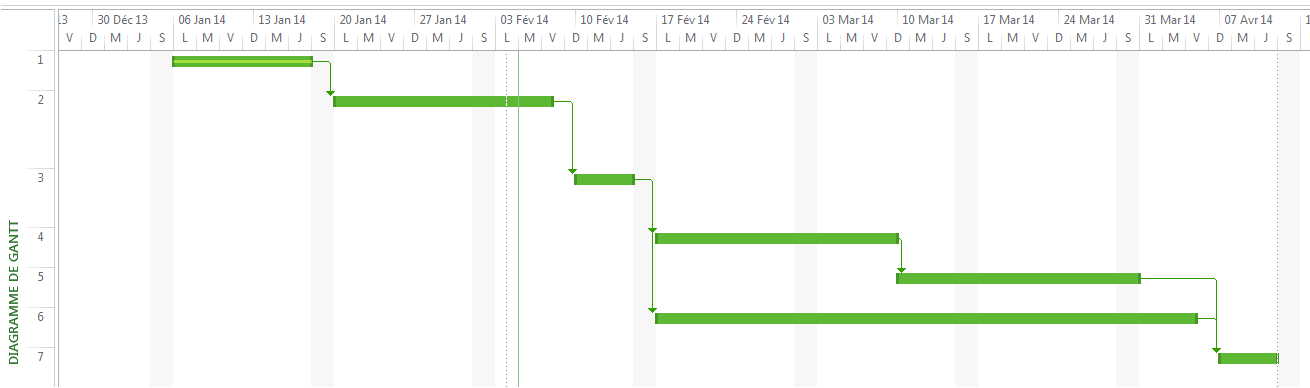
\includegraphics[scale=0.5]{gantt.png}
  \caption{Diagramme de GANTT représentant la gestion du temps pour le projet.}
  \label{diag-gantt}
\end{figure}

\begin{table}[H]
  \resizebox{0.7\textwidth}{2cm}{\begin{minipage}{\textwidth}
      \begin{tabular}{|c|c|c|c|c|c|}
        \hline
        Numéro de Tâche & Nom de la tâche & Durée & Début & Fin & Prédécesseurs \tabularnewline
        \hline
        1 & Bibliographie + Analyse de l'existant & 10 jours & Lun 06/01/14 & Ven 17/01/14 &  \tabularnewline
        \hline
        2 & Rédaction du Cahier des Besoins + Etablissement des Tests & 15 jours & Lun 20/01/14 & Ven 07/02/14 & 1 \tabularnewline
        \hline
        3 & Mise en place de l'architecture Logicielle & 5 jours & Lun 10/02/14 & Ven 14/02/14 & 2 \tabularnewline
        \hline
        4 & Développement logiciel + Tests & 16 jours & Lun 17/02/14 & Dim 09/03/14 & 3 \tabularnewline
        \hline
        5 & Tests (Débug logiciel)  & 16 jours & Lun 10/02/14 & Dim 30/03/14 & 4 \tabularnewline
        \hline
        6 & Rédaction du mémoire de projet & 35 jours & Lun 17/02/14 & Ven 04/04/14 & 3 \tabularnewline
        \hline
        7 & Préparation et entraînement pour la soutenance & 5 jours & Lun 07/04/14 & Ven 11/04/14 & 5;6  \tabularnewline
        \hline
      \end{tabular}
      \caption{\label{tab}Tableau descriptif des tâches}
    \end{minipage}}
\end{table}

\begin{enumerate}
\item L'analyse de l'existant permet de commencer le projet, et de réaliser une ébauche de la bibliographie qui sera complétée (modifiée) lors de la rédaction du mémoire final de projet.
\item Rédaction du cahier des Besoins (Fonctionnels et Non-fonctionnels). Etablissement des tests à réaliser pendant et après la phase de développement.
\item Réalisation de l'architecture logicielle. Modélisation à l'aide du logiciel UML Designer.
\item Le développement logiciel contient les tâches suivantes :
  \begin{itemize}
  \item Réalisation de l'IHM 
  \item Réalisation de la gestion des fichiers (pour la sauvegarde d'une partie)
  \item Réalisation de l'Intelligence Artificielle du jeu
  \end{itemize}
  Durant toute la durée de développement logiciel, les tests sont réalisés.
\item Réalisation des tests sur le logiciel afin de traquer les bugs existants.
\item La rédaction du mémoire de projet est répartie sur la durée du développement et des tests. La durée estimée est d'une semaine pour les quatre membres du projet.
\item  Cette partie du projet consiste à la réalisation d'un support de présentation (Power Point). Nous allons aussi réaliser des entraînements de soutenance.
\end{enumerate}

\subsection{Besoins Externes}

\subsubsection{Contraintes d'interopérabilité}

Aucune contrainte.

\subsubsection{Contraintes légales}

Aucune contrainte.

\subsubsection{Contraintes éthiques}

L'IA ne doit pas pouvoir gagner 5 parties de suite.

\appendix
\appendixpage
\addappheadtotoc 

\section{Diagramme de déploiement}
\label{A}
\begin{figure}[H]
  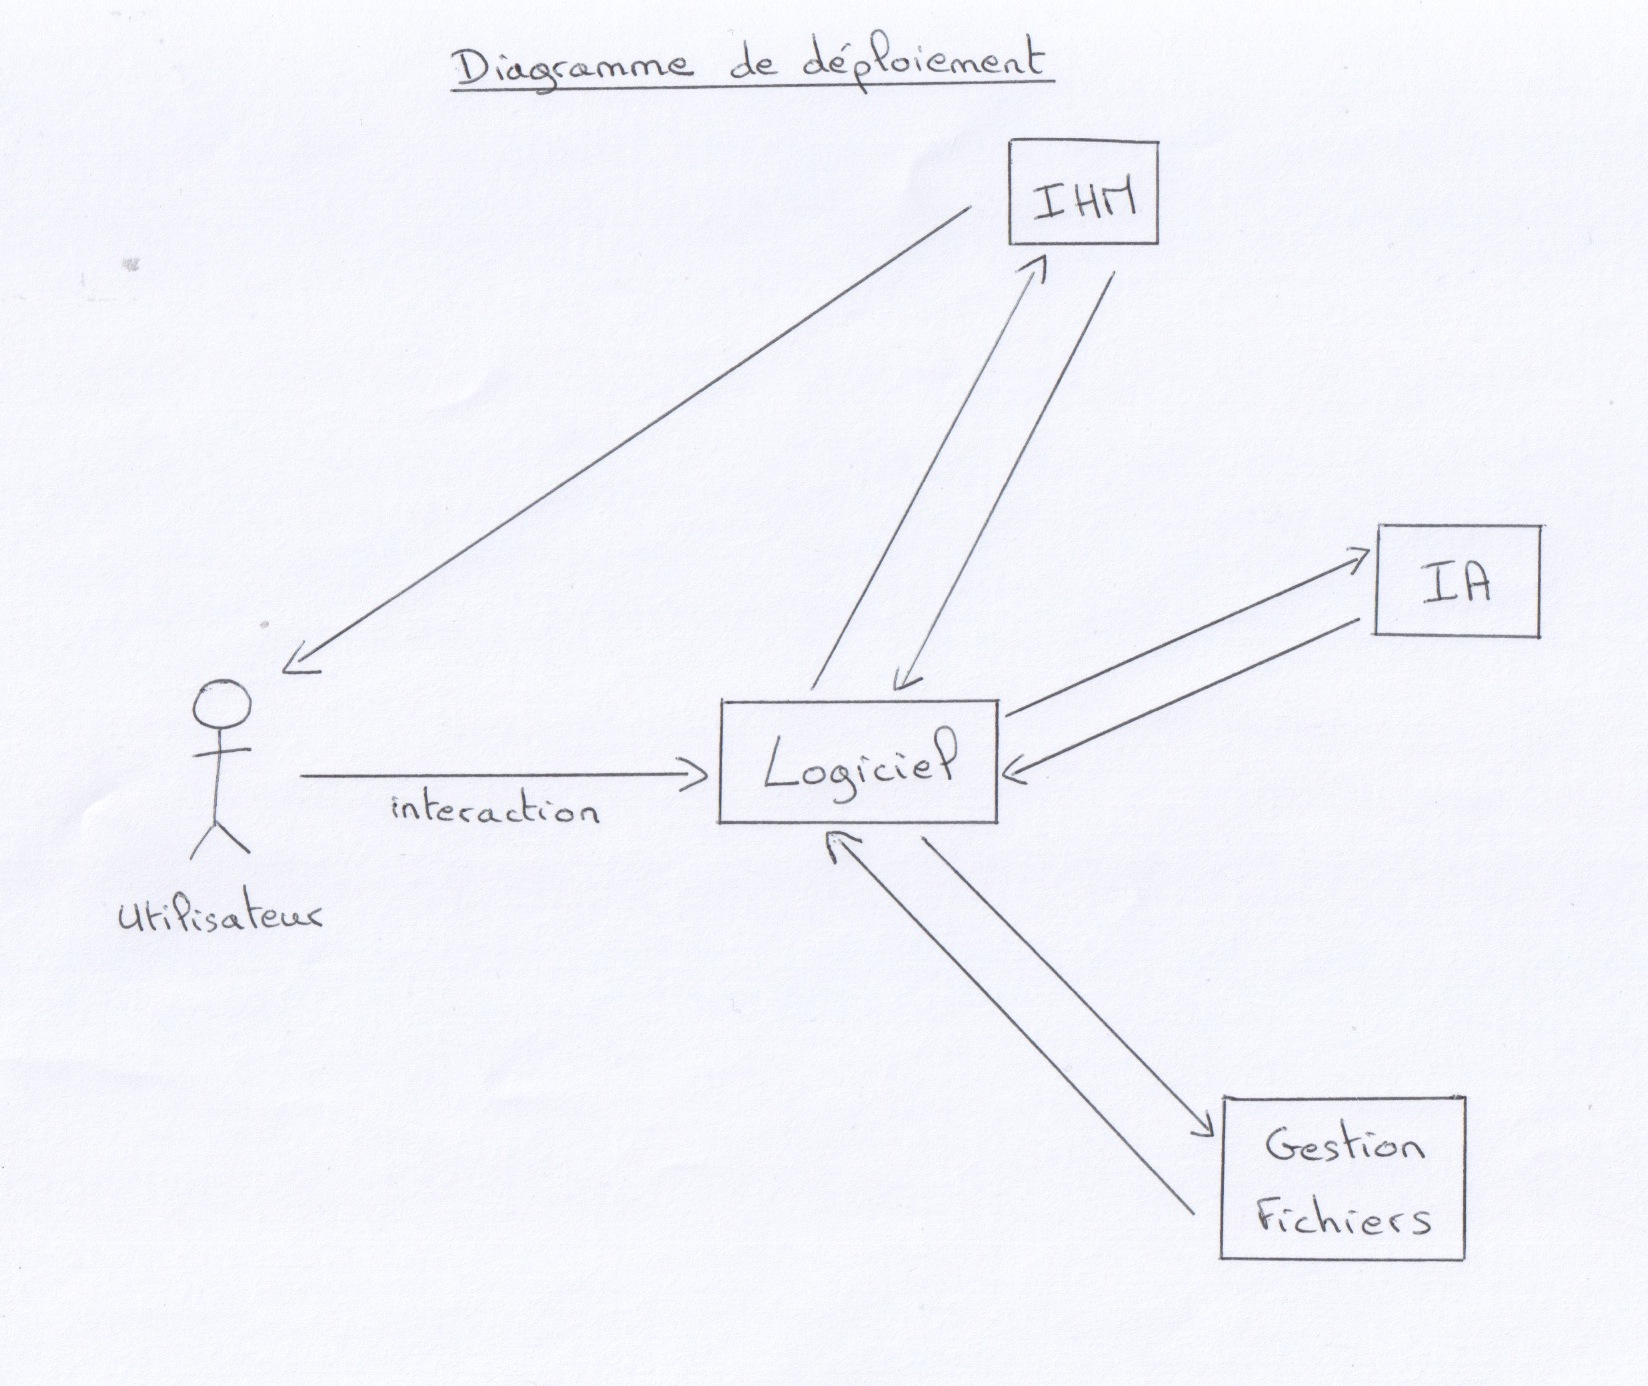
\includegraphics[scale=0.8]{deploiement.jpeg}
\caption{Diagramme UML de déploiement}
\label{deploi}
\end{figure}

\section{Diagramme des cas d'utilisation}
\label{B}
\begin{figure}[H]
  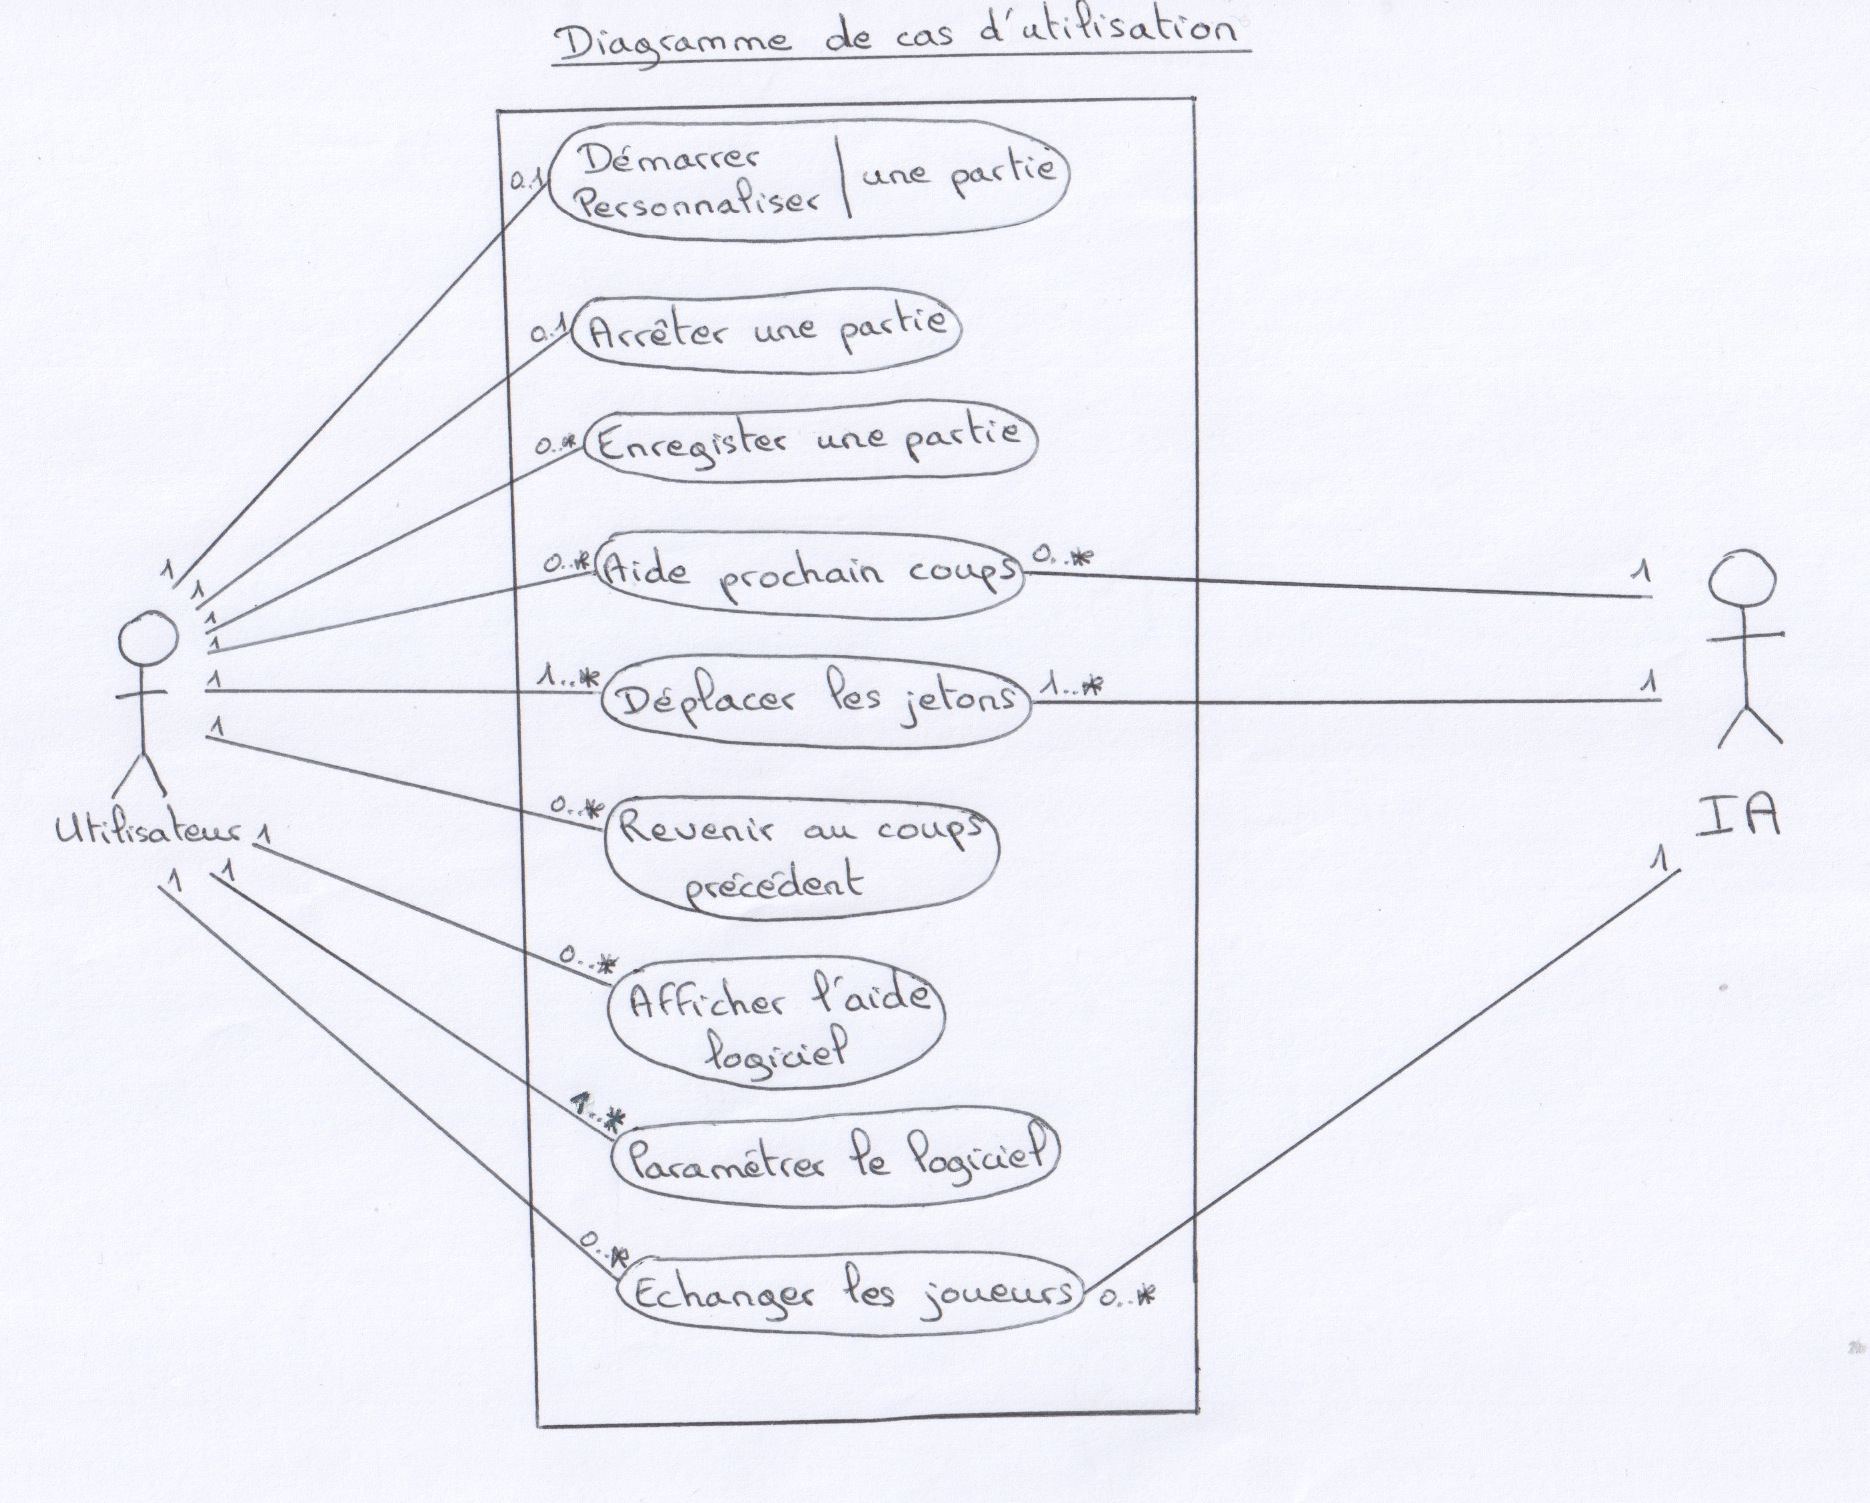
\includegraphics[scale=0.7]{cas-utilisation.jpeg}
\caption{Diagramme UML des cas d'utilisation du logiciel}
\label{cas}
\end{figure}


\section{Diagramme de machine à états}
\label{C}
\begin{figure}[H]
  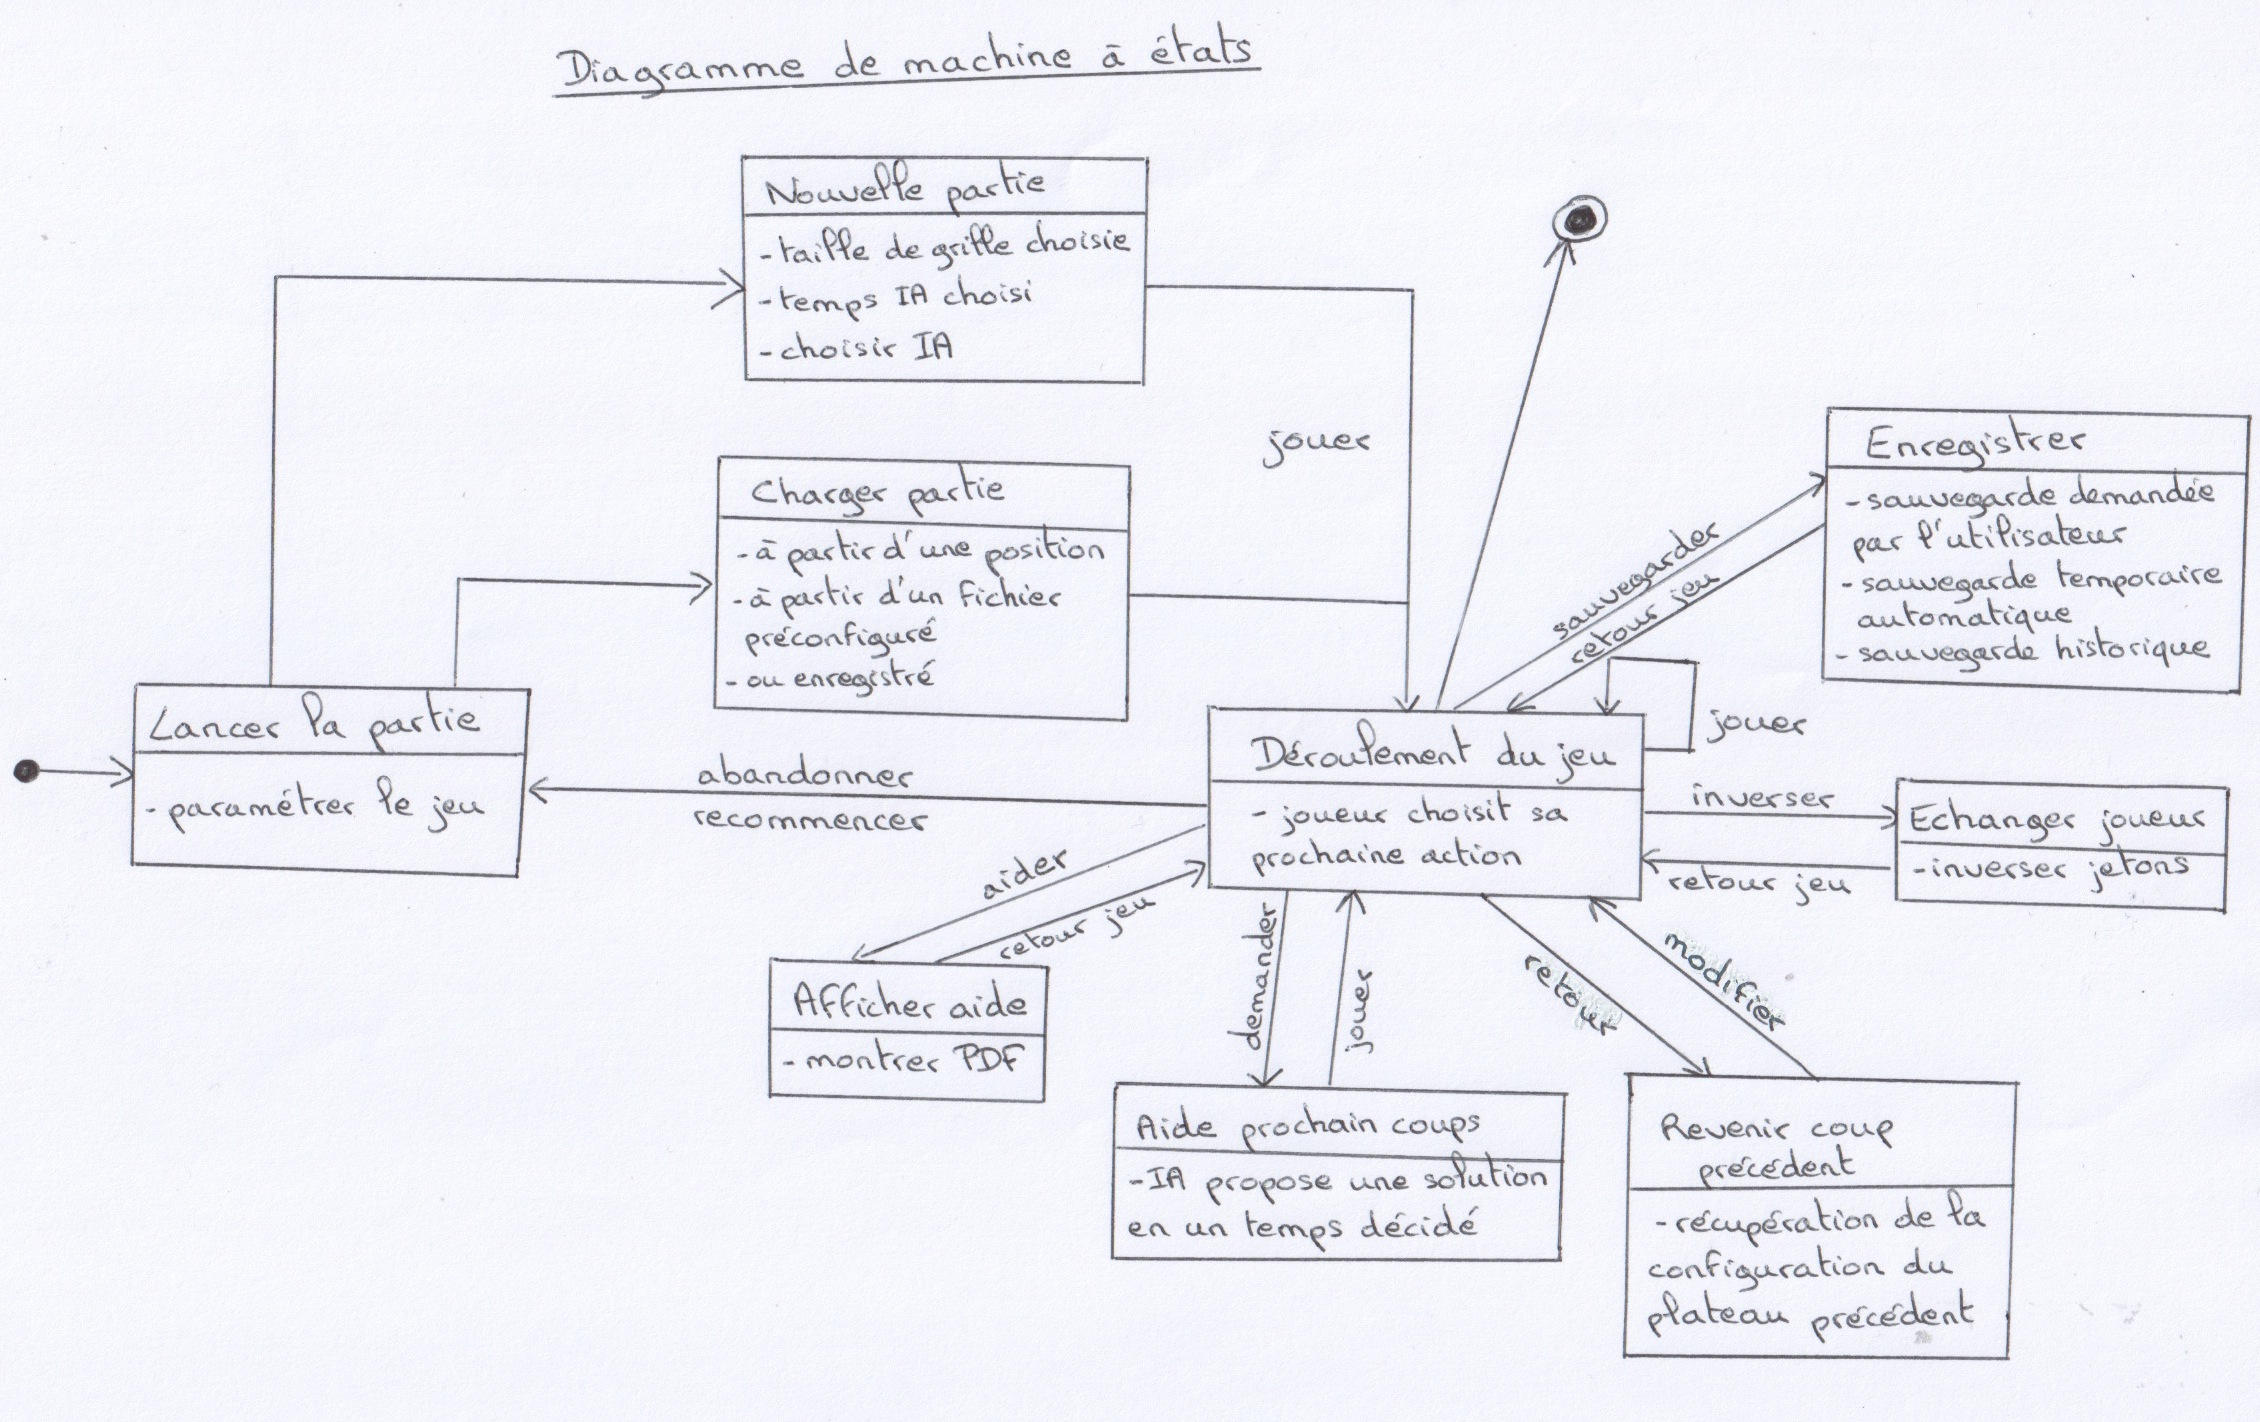
\includegraphics[scale=0.6]{machine-etat.jpeg}
\caption{Diagramme UML de machine à états}
\label{etat}
\end{figure}


\section{Prototypes papier de l'interface}
\label{D}

\begin{figure}[H]
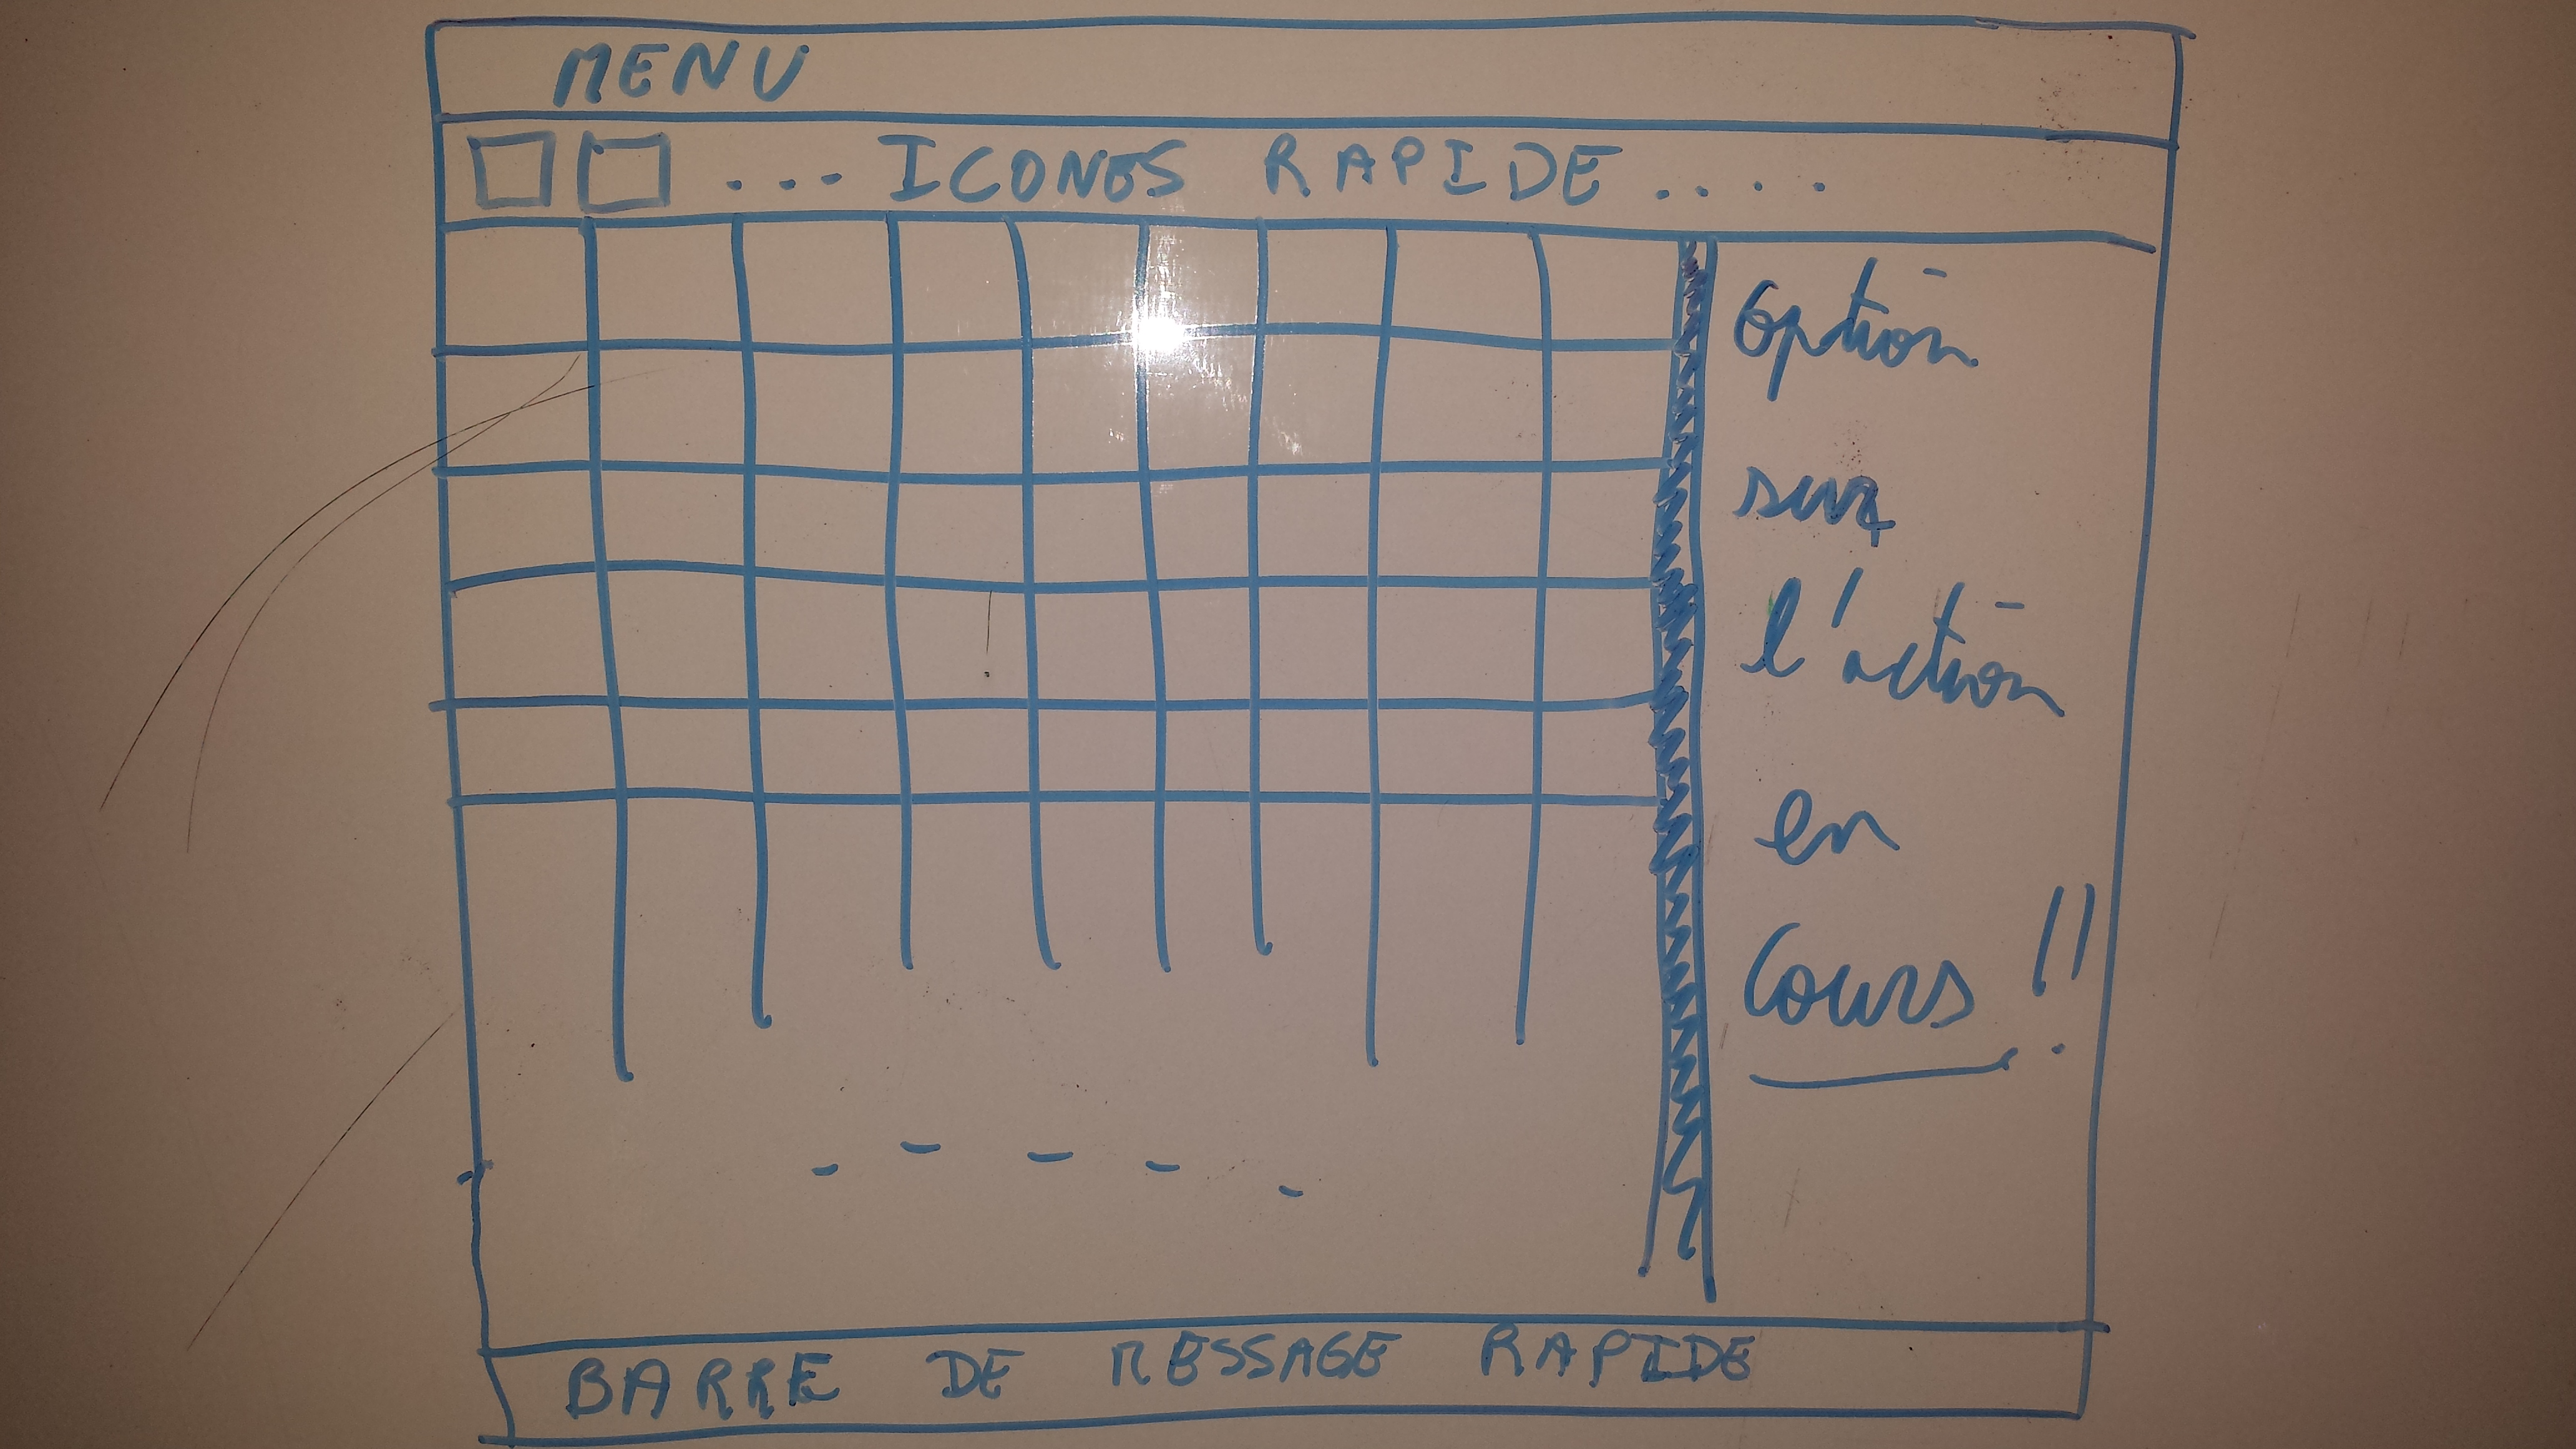
\includegraphics[scale=0.1]{plateau.jpg}
\caption{Plateau de jeu comprenant la grille, les menus et les
  boutons}
\label{plateau}
\end{figure}

\begin{figure}[H]
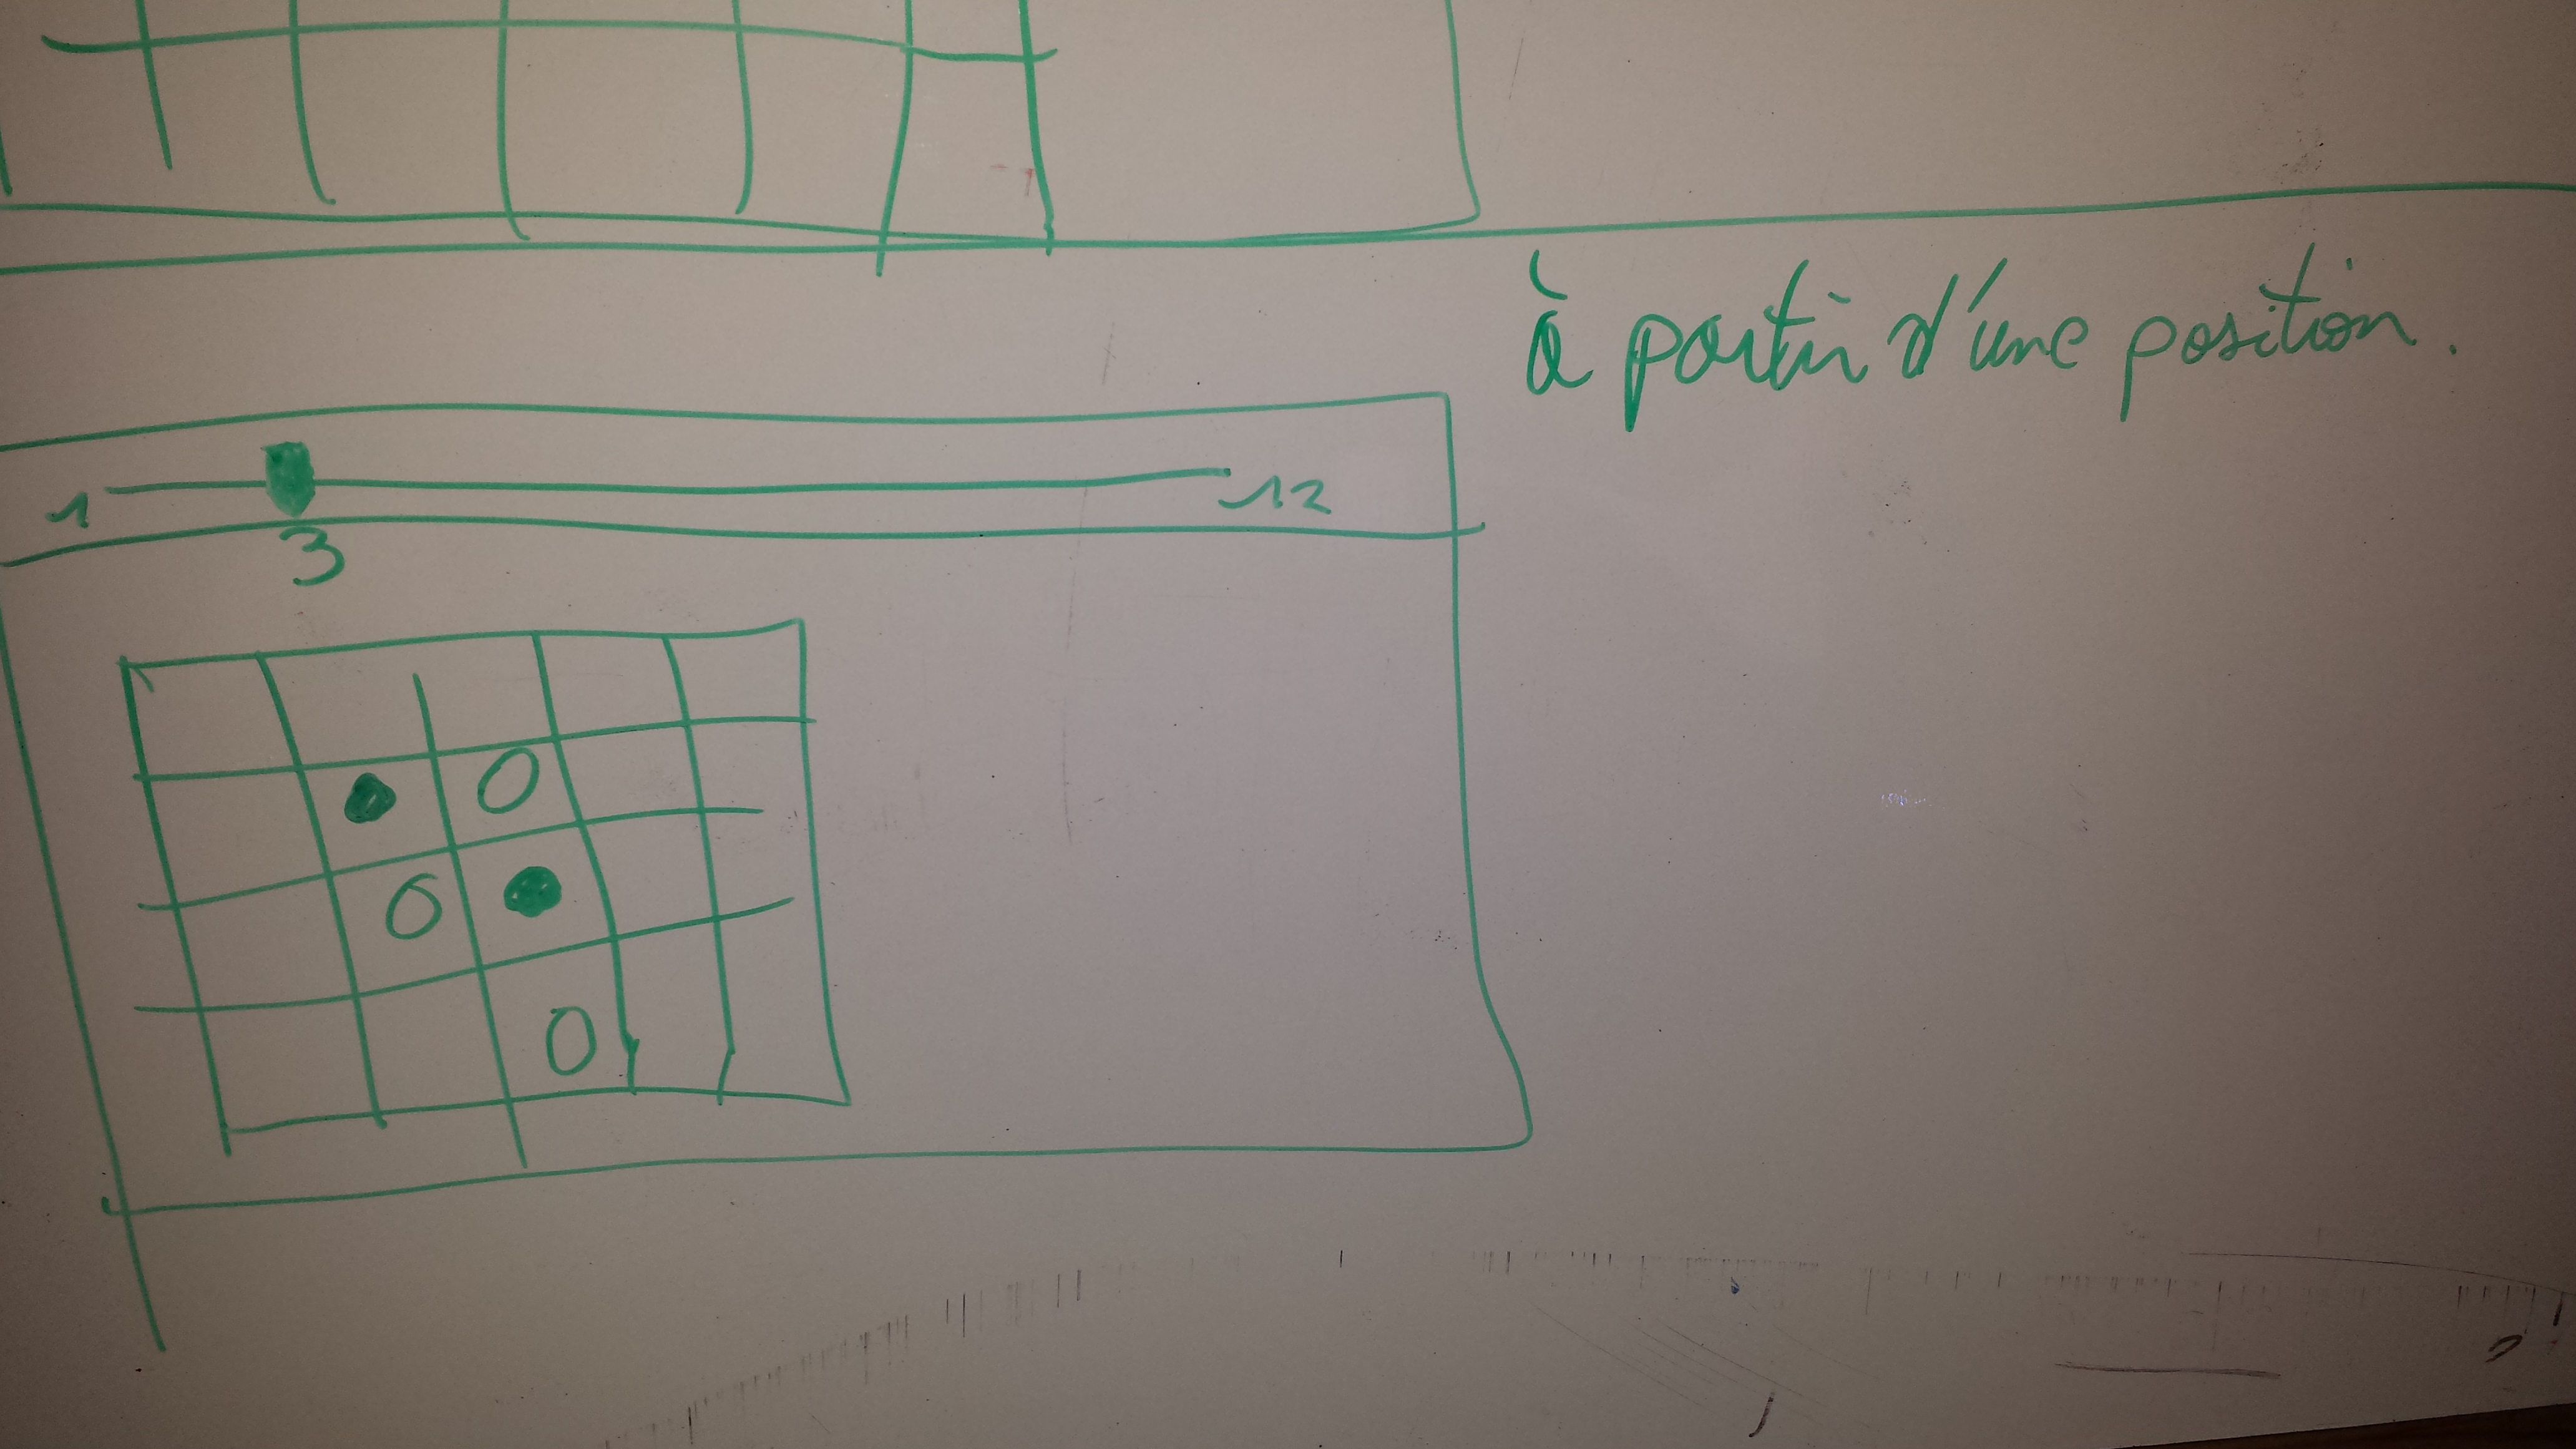
\includegraphics[scale=0.1]{position.jpg}
\caption{Prototype de la fonctionnalité de retour en arrière pour des coups}
\label{retour}
\end{figure}

\begin{figure}[H]
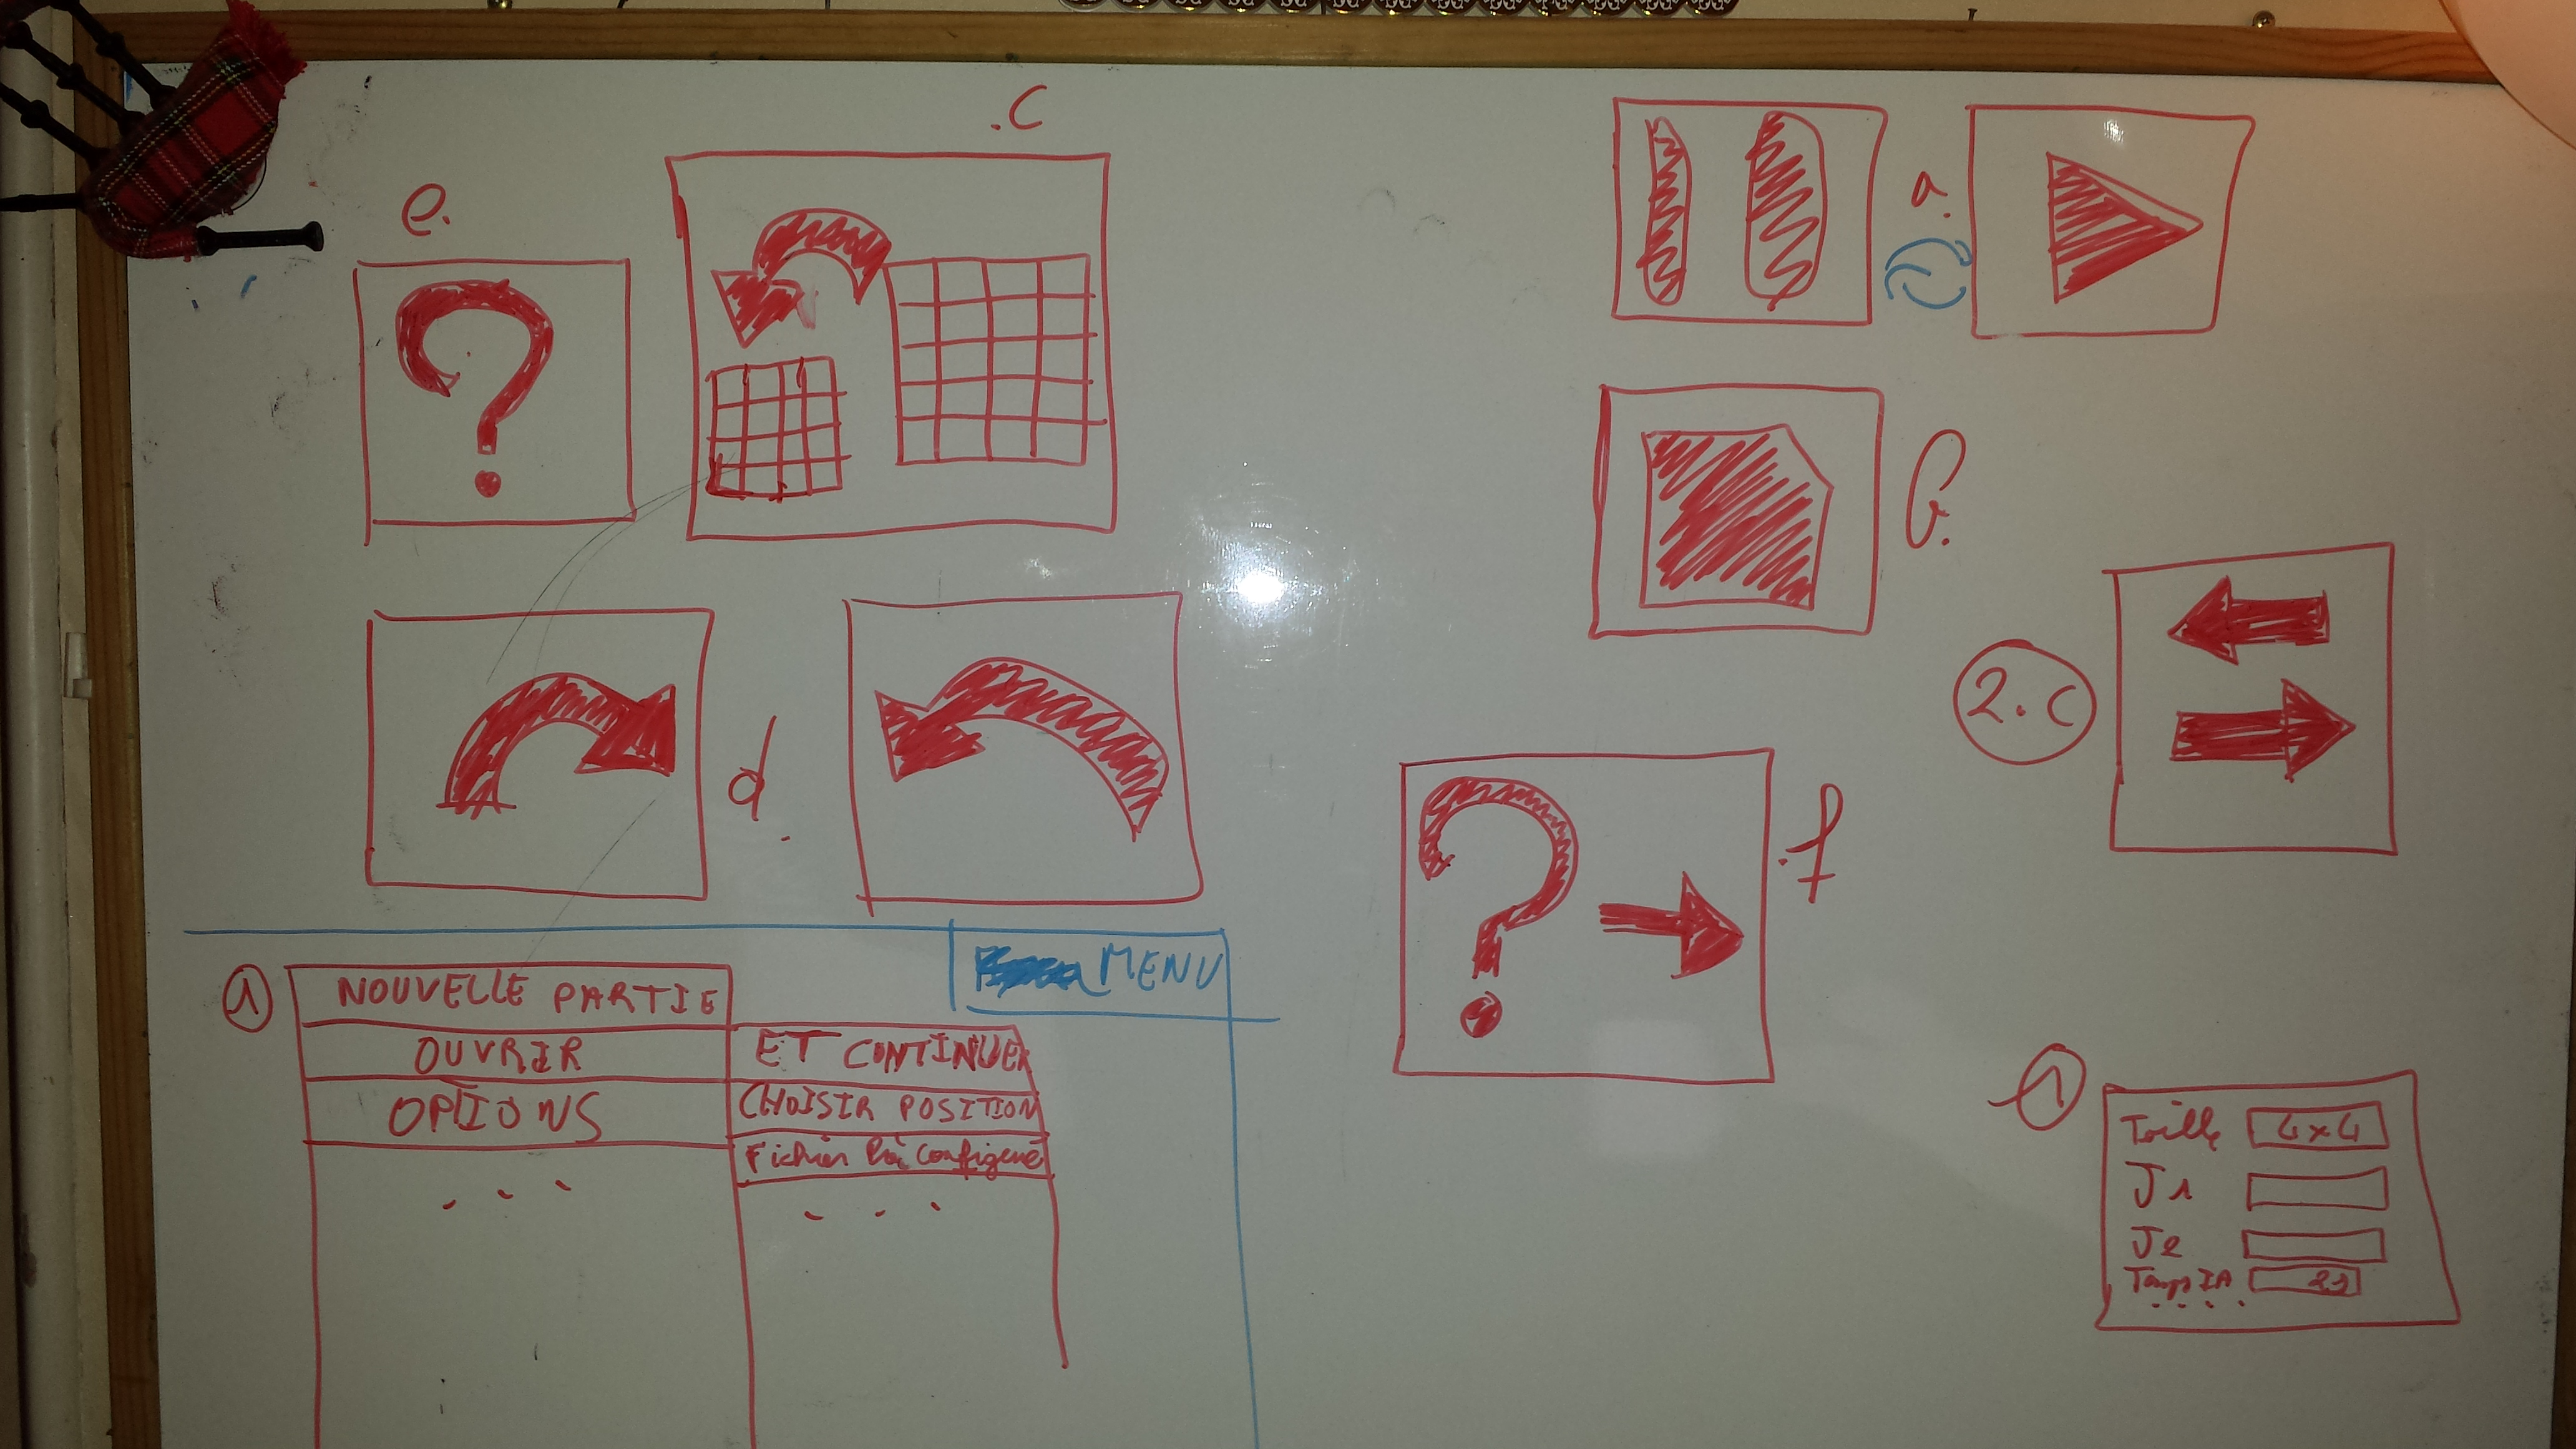
\includegraphics[scale=0.1]{boutons.jpg}
\caption{Prototype des boutons et des menus pour l'interface}
\label{boutons}
\end{figure}

\end{document}


